
\hypertarget{working_findreplace}{}
\section{Find and replace}
\index{find and replace}

\begin{figure}[h!]
  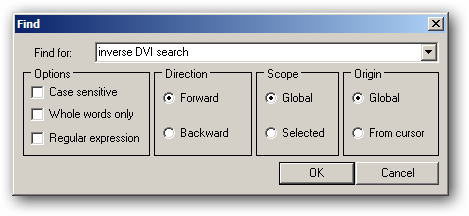
\includegraphics[scale=0.35]{./res/find.png}~~
  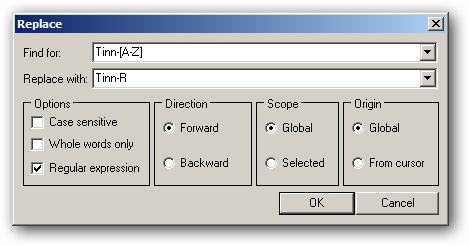
\includegraphics[scale=0.35]{./res/replace.png}\\
  \caption{Find and replace dialog.}
  \label{fig:find_replace}
\end{figure}

The dialogs for \textit{Find}
and \textit{Replace}
(Figure \ref{fig:find_replace})
are very similar, so this session will just discuss the \textit{Replace} dialog
and will point out the changes when necessary.


\subsection{Find}
\index{find}

When you call up the \textit{Find} dialog
the \textit{Find for} box will be
prefilled with the word under the cursor. You can type over the entry if you
are looking for another word. There is also a dropdown list of phrases
previously searched.


\subsection{Replace (Replace dialog only)}
\index{replace}

When you call up the \textit{Replace} dialog
the \textit{Replace with} box
will be filled with the last string you entered in it. If this is the first
time you have called the \textit{Replace} dialog since starting Tinn-R then
the Replace box will be empty. You can type over any text in box. There is
also a dropdown list of strings previously used.


\subsubsection{Options:}

\begin{quote}
  \begin{footnotesize}
    \begin{description}
      \item[Case sensitive:]
        When this option is set the search is done case sensitively. For instance,
        \texttt{Ab}, \texttt{AB} and \texttt{ab} are all treated as different words
        whereas they are not if the option is not set.
      \item[Whole words only:]
        When this option is set the system will only find complete words matching
        the search criteria. So, for example, if \texttt{ab} is the search string
        the system will not match occurrences of words like \texttt{abc} or
        \texttt{cab}.
      \item[Regular expressions:]
        \htmladdnormallink{See regular expressions ...}{\#working\_regularexpressions}
    \end{description}
  \end{footnotesize}
\end{quote}


\subsubsection{Direction:}

The direction to search. This option is ignored if searching in selected text.

\begin{quote}
  \begin{footnotesize}
    \begin{description}
      \item[Forward:]
        Search from the cursor position to the end of the file.
      \item[Backward:]
        Search from the cursor position to the beginning of the file.
    \end{description}
  \end{footnotesize}
\end{quote}


\subsubsection{Scope:}
\begin{quote}
  \begin{footnotesize}
    \begin{description}
      \item[Global:]
        Search the entire file.
      \item[Selected Text:]
        Search just the selected text.
    \end{description}
  \end{footnotesize}
\end{quote}


\subsubsection{Origin:}
\begin{quote}
  \begin{footnotesize}
    \begin{description}
      \item[Global:]
        Search from the beginning of the file.
      \item[From cursor:]
        Search just from the position of the cursor.
    \end{description}
  \end{footnotesize}
\end{quote}
